\documentclass[twoside]{article} 
\usepackage{amsmath}
\usepackage{amsfonts}
\usepackage[pdftex]{graphicx}
\usepackage[procnames]{listings}
\usepackage{color}
\usepackage{lipsum} % Package to generate dummy text throughout this template
\usepackage{braket}
\usepackage{epsfig}
\usepackage{epstopdf}


\usepackage[sc]{mathpazo} % Use the Palatino font
\usepackage[T1]{fontenc} % Use 8-bit encoding that has 256 glyphs
\linespread{1.05} % Line spacing - Palatino needs more space between lines
\usepackage{microtype} % Slightly tweak font spacing for aesthetics

\usepackage[hmarginratio=1:1,top=32mm,columnsep=20pt]{geometry} % Document margins
\usepackage{multicol} % Used for the two-column layout of the document
\usepackage[width=.8\textwidth,hang, small,labelfont=bf,up,textfont=it,up]{caption} % Custom captions under/above floats in tables or figures
\usepackage{float} % Required for tables and figures in the multi-column environment - they need to be placed in specific locations with the [H] (e.g. \begin{table}[H])
\usepackage{hyperref} % For hyperlinks in the PDF

\usepackage{lettrine} % The lettrine is the first enlarged letter at the beginning of the text
\usepackage{paralist} % Used for the compactitem environment which makes bullet points with less space between them

\newcommand{\unit}[1]{\ensuremath{\; \mathrm{#1}}}

\usepackage{abstract} % Allows abstract customization
\renewcommand{\abstractnamefont}{\normalfont\bfseries} % Set the "Abstract" text to bold
\renewcommand{\abstracttextfont}{\normalfont\small\itshape} % Set the abstract itself to small italic text

\usepackage{titlesec} % Allows customization of titles
\renewcommand\thesection{\arabic{section}} % Roman numerals for the sections
\renewcommand\thesubsection{\thesection.\arabic{subsection}} % Roman numerals for subsections
\titleformat{\section}[block]{\large\scshape\centering}{\thesection.}{1em}{} % Change the look of the section titles
\titleformat{\subsection}[block]{\large}{\thesubsection.}{1em}{} % Change the look of the section titles

\usepackage{fancyhdr} % Headers and footers
\pagestyle{fancy} % All pages have headers and footers
\fancyhf{}
\fancyhead[C]{Molecular Dynamics Simulation of a Lenard-Jones Interacting Molecule for Obtaining Macroscopic Static Physical Properties $\bullet$ February 2016} % Custom header text
\fancyfoot[RO,LE]{\thepage} % Custom footer text
\fancyfoot[CO,CE]{Jaap Wesdorp \& Bas Dirkse}
\fancypagestyle{firststyle}
{	
	\fancyhf{}
	\renewcommand{\headrulewidth}{0pt}
	\fancyfoot[RO,LE]{\thepage}
	\fancyfoot[CO,CE]{Jaap Wesdorp \& Bas Dirkse}
}

\usepackage{subcaption}
\captionsetup{compatibility=false}

%----------------------------------------------------------------------------------------
%	TITLE SECTION
%----------------------------------------------------------------------------------------

\title{\vspace{-15mm}\fontsize{18pt}{10pt}\selectfont\textbf{Computation of the Ground State Energy of the Hydrogen Molecule using the Variational Monte Carlo Method}} % Article title

\author{
	\large
	\textsc{Jaap Wesdorp}$^\dagger$, $\hspace{10pt}$ \textsc{Bas Dirkse}$^\dagger$ \\ % Your name
	\normalsize $^\dagger$Delft University of Technology \\ % Your institution
	\normalsize \href{mailto:j.j.wesdorp@student.tudelft.nl}{j.j.wesdorp@student.tudelft.nl} \\
	\normalsize \href{mailto:b.dirkse@student.tudelft.nl}{b.dirkse@student.tudelft.nl} 
}
\date{\today\vspace{-8mm}}

%----------------------------------------------------------------------------------------

\newcommand{\bfr}{\ensuremath{\mathbf{r}}}


\begin{document}

\definecolor{keywords}{RGB}{255,0,90}
\definecolor{comments}{RGB}{0,0,113}
\definecolor{red}{RGB}{160,0,0}
\definecolor{green}{RGB}{0,150,0}

\lstset{language=Python, 
	basicstyle=\ttfamily\small, 
	keywordstyle=\color{keywords},
	commentstyle=\color{comments},
	stringstyle=\color{red},
	showstringspaces=false,
	identifierstyle=\color{green},
	procnamekeys={def,class}}

\maketitle % Insert title
\thispagestyle{firststyle} % Only footer on first page

%----------------------------------------------------------------------------------------
%	ABSTRACT
%----------------------------------------------------------------------------------------

\begin{abstract}
\noindent  
Some abstact

	
\end{abstract}

%----------------------------------------------------------------------------------------
%	ARTICLE CONTENTS
%----------------------------------------------------------------------------------------

\section{Introduction}
Solving the Schr\"odinger equation of interacting body systems has proved to be a formidable task and has not been done analytically for systems with more then a few particles. In this paper we approximate the ground state energy of the hydrogen molecule taking all coulomb interactions into account. A variational Monte Carlo method  is used to find the ground state wavefunction as described in Chapter \ref{ch_methods}. In Chapter \ref{ch_results} we describe the results and compare them to literature values and the well known Hartree fock approximation using product states. 

%------------------------------------------------

\section{Methods}\label{ch_methods}
 In the variational method for finding the ground state of the hydrogen molecule, we try to minimize the ground state energy from our system hamiltionian, described in section \ref{sec:hamiltonian}, by varying parameters of our trial wavefunction of section \ref{sec:wavefunc}. The computation of the expectation value of the energy from section \ref{sec:localEnergy} is done using the Metropolis Monte Carlo method described in \ref{sec:metropolis}, thereby avoiding the need to normalize the trial wave function and explicit integration in six dimensions. A a final step we optimize the variational parameters to find the ground state within our variational subspace. This is done by a gradient descent method described in \ref{sec:paramaterOptimization}. A full summary of the algorithm and parameters used is then given in section \ref{sec:algorithm}

\subsection{Natural Units of Computation}\label{sec:au}
In our computation we naturally use atomic units. For the distance, we use the unit of Bohr radius
\begin{equation}
a_0 = \frac{4\pi \varepsilon_0 \hbar^2}{me^2} \approx 0.529 \times 10^{-10} \unit{m},
\end{equation}
and for energy we use the Hartree unit
\begin{equation}
E_0 = \frac{m}{\hbar^2} \left(\frac{e^2}{4\pi \varepsilon_0}\right)^2 \approx 27.2 \unit{eV}. 
\end{equation}

\subsection{The Hamiltonian of the Hydrogen Molecule}\label{sec:hamiltonian}
In this paper we approximate the Hydrogen molecule system as two stationary protons separated by a distance $s$, supplemented with two electrons. We choose our coordinate system such that both protons are symmetrically located around the origin and positioned on the x-axis, i.e. the protons are at $[\pm s/2,0,0]^T$. The Hamiltonian of this system includes the kinetic energy of the electrons, the potential energy of each electron due to the two protons, an electron-electron interaction term and the proton-proton interaction term. Let the positions of the electrons be given by $\bfr_1$ and $\bfr_2$ respectively. In our natural units, the Hamiltonian is then given by
\begin{equation}
H = -\frac{1}{2} (\nabla_1^2 + \nabla_2^2) - \left[ \frac{1}{r_{1L}} + \frac{1}{r_{1R}} + \frac{1}{r_{2L}} + \frac{1}{r_{2R}}  \right] + \frac{1}{r_{12}} + \frac{1}{s},
\end{equation}
where
\begin{equation}
\begin{split}
&\bfr_{iL} = \bfr_i + \frac{s}{2} \mathbf{\hat{x}}; \quad\quad \bfr_{iR} = \bfr_i - \frac{s}{2} \mathbf{\hat{x}}; \quad \quad i=1,2; \quad \mbox{and} \\
&\bfr_{12} = \bfr_1 - \bfr_2.
\end{split}
\end{equation}

\subsection{The Variational Wave Function}\label{sec:wavefunc}
The variational form of the wave functions is chosen to be of the following form
\begin{equation}
\Psi(\bfr_1,\bfr_2) = \phi_1(\bfr_1)\phi_2(\bfr_2)\psi(\bfr_1,\bfr_2),
\end{equation}
where 
\begin{equation}
\phi_i(\bfr_i) = e^{-r_{iL/a}} + e^{-r_{iR/a}} = \phi_{iL}(\bfr_i) + \phi_{iR}(\bfr_i), \quad i=1,2.
\end{equation}
Note that these parts are just the sum of the wave functions of each electron being in the ground state of the left or right hydrogen atom. The interaction part of the wave function is chosen to be the Jastrow function
\begin{equation}
\psi(\bfr_1,\bfr_2) = \exp\left[ \frac{r_{12}}{\alpha(1+\beta r_{12})} \right].
\end{equation}
Note that we now have four variational parameters $a$, $s$, $\alpha$ and $\beta$. Later we will put constraints on two of these parameters to ensure that the expectation value of the energy remains bounded.

\subsection{The Local Energy}\label{sec:localEnergy}
The expectation value of the energy is computed using the local energy and a weight function. The weight function is then incorporated using the Metropolis Monte Carlo method, so that the expectation value of the energy is the integral of the local energy using points sampled from the weight function distribution. We thus compute the energy as
\begin{equation}
E = \frac{\braket{\Psi|H|\Psi}}{\braket{\Psi|\Psi}} = 
\iint \frac{\Psi^* H \Psi}{\braket{\Psi|\Psi}}  \; d^3\bfr_1 \; d^3\bfr_2 = 
\iint \frac{\Psi\Psi^*}{\braket{\Psi|\Psi}} \frac{H \Psi}{\Psi} \; d^3\bfr_1 \; d^3\bfr_2 = \iint \omega \varepsilon \; d^3\bfr_1 \; d^3\bfr_2,
\label{eq:ExpectedEnergy}
\end{equation} 
where
\begin{equation}
\omega(\bfr_1,\bfr_2) = \frac{|\Psi|^2}{\braket{\Psi|\Psi}},
\end{equation}
is the weight function and
\begin{equation}
\varepsilon(\bfr_1,\bfr_2) = \frac{H \Psi}{\Psi}
\label{eq:LocalEnergy}
\end{equation}
is the local energy. Note that intially both expressions depend on the positions $\bfr_1$ and $\bfr_2$, and also on the variational parameters. As $\Psi$ nears the ground state wavefunction, the local energy will become constant as can be seen from \eqref{eq:LocalEnergy}, so the variation of the local energy  over space gives a criterium for the needed amount of walker steps during the Monte-Carlo loop. Furthermore, note that $\omega$ is a normalized probability distribution, which is very useful for the integration of \eqref{eq:ExpectedEnergy}.

Plugging in the variational wave function and the Hydrogen molecule Hamiltonion into \eqref{eq:LocalEnergy} we find an expression for the local energy in our problem
\begin{equation}
\begin{split}
\varepsilon(\bfr_1,\bfr_2) &= 
-\frac{1}{a^2} 
+ \frac{1}{a\phi_1} \left(\frac{\phi_{1L}}{r_{1L}} + \frac{\phi_{1R}}{r_{1R}}\right) 
+ \frac{1}{a\phi_2} \left(\frac{\phi_{2L}}{r_{2L}} + \frac{\phi_{2R}}{r_{2R}}\right)
- \left( \frac{1}{r_{1L}}+\frac{1}{r_{1R}}+\frac{1}{r_{2L}}+\frac{1}{r_{2R}} \right) + \frac{1}{s} \\
&+ \frac{1}{r_{12}} 
+ \left( \frac{\phi_{1L}\hat{\bfr}_{1L} + \phi_{1R}\hat{\bfr}_{1R}}{\phi_1} - \frac{\phi_{2L}\hat{\bfr}_{2L} + \phi_{2R}\hat{\bfr}_{2R}}{\phi_2} \right) \cdot \frac{\hat{\bfr}_{12}}{2a(1+\beta r_{12})^2} 
- \frac{(4\beta+1)r_{12}+4}{4(1+\beta r_{12})^4 r_{12}}. 
\end{split}
\end{equation}
At this point we can eliminate two variational parameters by imposing the so-called Coulomb cusp conditions. These conditions are required to ensure that the energy does not blow up when either electron approaches either proton, or when the two electrons approach each other. The four cases of an electron approaching a proton leads to the same condition $a(1+e^{-s/a}) = 1$. The case of the two electrons approaching each other leads to the condition $\alpha = 2$.

\subsection{Metropolis Monte Carlo Integration}\label{sec:metropolis}
To evaluate the integral \eqref{eq:ExpectedEnergy} we use the Metropolis Monte Carlo method. In this method we choose random positions $\bfr_1^i$ and $\bfr_2^i$ from the distribution $\omega$ and approximate the integral as
\begin{equation}
\iint \omega \varepsilon \; d^3\bfr_1 \; d^3\bfr_2 \approx \frac{1}{NT} \sum_{i=1}^{NT} \varepsilon(\bfr_1^i,\bfr_2^i) = \braket{\varepsilon},
\end{equation}
where $NT$ is the total number of configurations, and $\braket{...}$ denotes the average over all configurations. The key is to generate a lot of points from the distribution $\omega$, which depends on $\Psi$, without having to normalize it. We can do this by generating a large set of points using a Markov Chain. We do this as follows:

Let $R$ denote the six dimensional coordinates of both electrons. We initialize the electrons at some random position, and repeatedly propose a new state $R'$. We accept the state with probability $p = \frac{|\Psi(R')|^2}{|\Psi(R)|^2}$. If $p > 1$ we always accept the new state and if the new state is rejected, then the old state $R$ is kept. 
This process is an ergodic Markov Chain and for large enough number of time steps, the collection of positions $R$ obtained in this way approximately satisfy the distribution $\omega(R)$. This is why we let the positions equilibrate for $T_0$ time steps and then do $T$ of such random walks in the state space, saving each position. This is done simultaneously for $N$ walkers, in order to avoid walkers getting stuck in local minima.

\subsection{Parameter optimization}\label{sec:paramaterOptimization}
So far we have described a way to find the expectation value of the energy for a proposed trial wave function given the Hamiltonian of the Hydrogen molecule. In order to obtain the ground state within the variational subspace, we must minimize this energy with respect to the variational parameters. As we have seen before, we effectively have 3 parameters and one constraint, after setting $\alpha = 2$. Perfect optimization with respect to the three parameters would lead to a constraint optimization problem. However, this is overly complicated, and in this paper we compute the energy for various $s$. Fixing $s$, yields $a$ from the constraint $a(1+e^{-s/a}) = 1$, leaving $\beta$ as the only free parameter. For this, we can just use a gradient descent method. Computing the derivative of the energy w.r.t. $\beta$ using a finite difference scheme would yield large errors due to the stochastic nature of the approach. However, this derivative can be computed differently. From \eqref{eq:ExpectedEnergy} we find\cite{ref_Harju}\cite{ref_Thijssen} 
\begin{equation}
\frac{\partial E}{\partial \beta} = 2\left( \Braket{\varepsilon \frac{\partial \ln \Psi}{\partial \beta}} - E\Braket{\frac{\partial \ln \Psi}{\partial \beta}} \right),
\end{equation}
which generally holds for any variational parameter $\beta$ and trial wave function $\Psi$. In our case we find that $\frac{\partial \ln \Psi}{\partial \beta} = -\frac{r_{12}^2}{2(1+\beta r_{12})}$.

\subsection{Algorithm overview}\label{sec:algorithm}
Here we briefly summarize the algorithm and highlight some implementation choices we made. The algorithm was performed as follows:

\begin{enumerate}
	\item Initiate $N$ walkers uniformly within a six-dimensional hypercube of side $2s + 4a$ centered around the origin.
	\item Update walkers $T_0$ times by proposing a displacement in each of the six coordinates from a normal distribution with mean $0$ and standard deviation $\frac{1}{2}$. Accept the proposed displacement with probability $p$.
	\item Update walkers $T$ times as above and save their positions. Compute $\varepsilon$ for all positions. From this find $E$, Var($\varepsilon$) and $\frac{\partial E}{\partial \beta}$.
	\item Update $\beta \leftarrow \beta - \gamma \frac{\partial E}{\partial \beta}$, where we use $\gamma = 10$. Repeat 1-4 until $|\frac{\partial E}{\partial \beta}| < e$, where $e$ is some tolerance on the magnitude of the derivative, which we choose to be $10^{-4}$.
\end{enumerate}
We used $N = 400$ walkers, which we updated each of the $T_0 = 4000$ iterations to equilibrate and then generated $T = 26000$ updates for each walker, obtaining $NT = 10.4 \times 10^6$ configurations. We varied $s$ between $1$ and $1.8$ and optimized $\beta$ for each s taking $\beta_{init} = 0.6$.
Note that the tolerance on the derivative is not all small. Firstly, note that the derivative is based on stochastic variables and may deviate from the exact result. Secondly, we note that small changes in $\beta$ have a very small effect on the ground state energy found. Finally we note that the choice of the step length $\gamma$ depends strongly on the initial guess of $\beta$ and its distance to the optimal value. 

%-------------------------------------------------------------------------
% % RESULTS
%-------------------------------------------------------------------------


\section{Results and discussion}\label{ch_results}
In Figure~\ref{fig:EvsS_optimalBeta} we have plotted the energy $E$ versus the separation distance $s$ for various $s$ at an optimal value of $\beta$, i.e. the value of $\beta$ that minimizes the energy at a given $s$. This value of $\beta$ is plotted on the right axis. Each calculation was repeated 5 times in order to obtain an estimate of the uncertainty in $E$, which is shown in error bars. We find a minimum energy of $E = -1.1510 \pm 0.0003$ at $s = 1.4 \pm 0.05$. The corresponding value for $\beta = 0.59 \pm 0.01$. 

We compare these values to experimental data found in literature\cite{ref_NIST}\cite{ref_Grinter}. We find a dissociation energy of $-4.477 \unit{eV}$ at $T=0 \unit{K}$, which in units of Hartree is $-0.1645$. Since the dissociation energy is the energy gain from forming the molecular bond from two separate hydrogen atoms, we add $-1$ Hartree to this for the ground state energy of two hydrogen atoms to arrive at a ground state energy for the Hydrogen molecule of $-1.1645$. Our result of $-1.1510 \pm 0.0003$ compares very well with the experimental result as compared to the Hartree Fock approximation which arrives at $-1.125$ Hartree. This indicates that the inclusion of the Jastrow function gives better approximation of the ground state wavefunction than just using a product state of independent wavefunctions. Furthermore the literature states a separation distance of $74.1 \unit{pm}$, which is $1.400$ Bohr radii. Our result agrees with this result.

Finally we observe that the optimal value of $\beta$ decreases linearly as the separation distance $s$ decreases, indicating the reduced interaction between the two electrons.

\begin{figure}
	\centering
	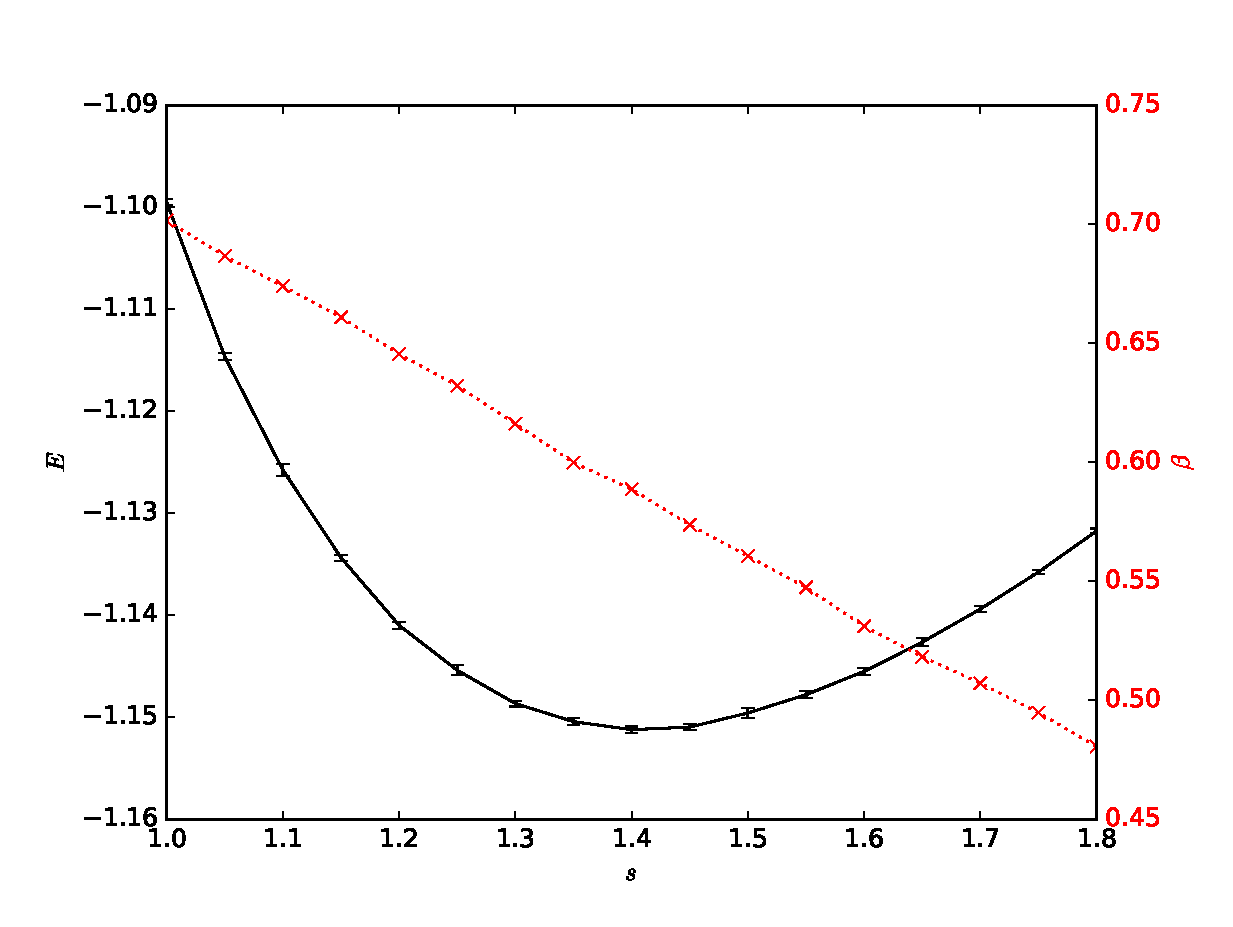
\includegraphics[width=0.8\linewidth]{figs/EvsS_optimalBeta.eps}
	\caption{Plot of the energy $E$ and $\beta$ versus the separation distance $s$, where $\beta$ is optimized to minimize the energy. The solid line shows the energy $E$ on the left axis and the dotted line shows the corresponding $\beta$ on the right axis, each as a function of $s$.}
	\label{fig:EvsS_optimalBeta}
\end{figure}

\begin{figure}
\centering
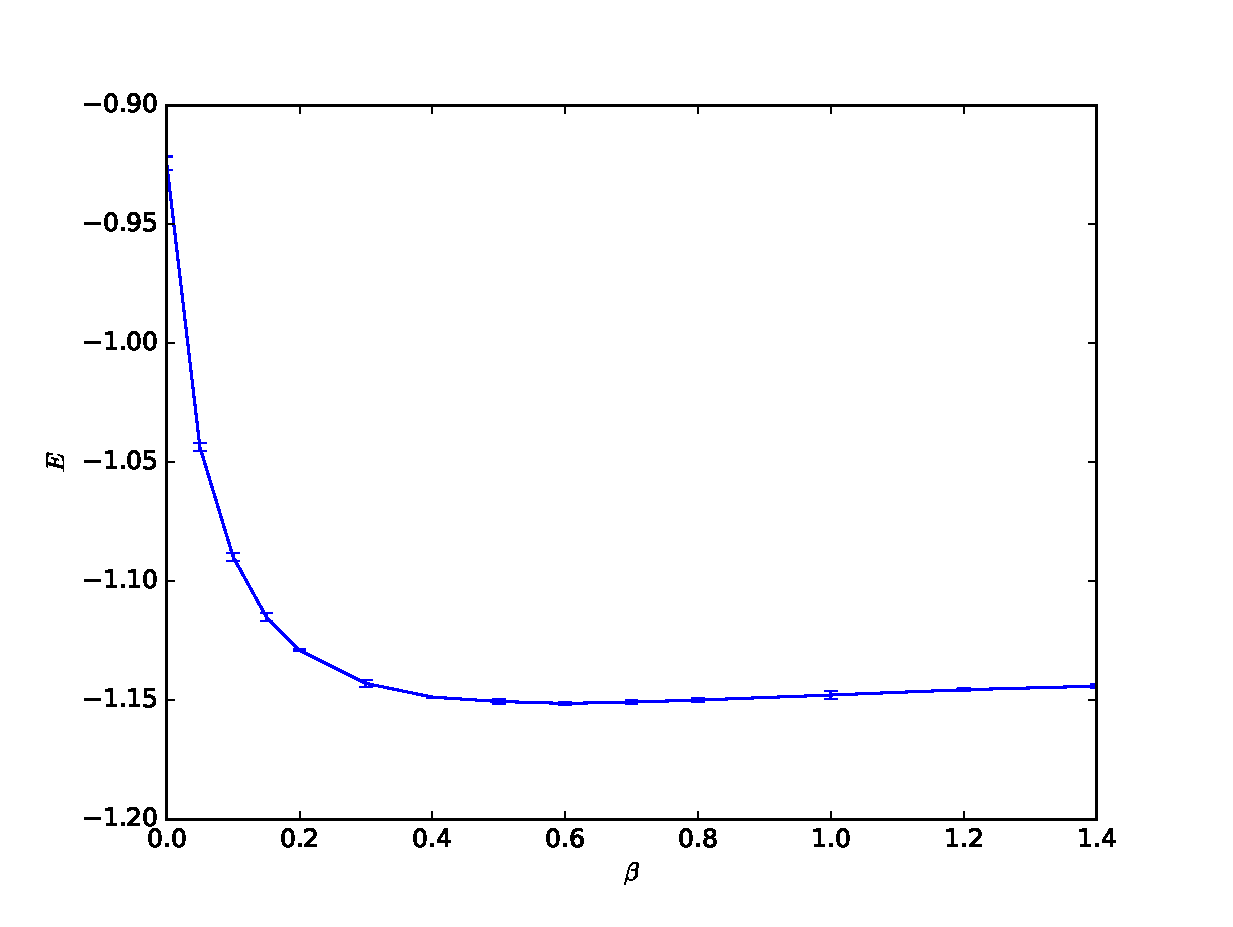
\includegraphics[width=0.8\linewidth]{figs/EvsBeta.eps}
\caption{Plot of the energy $E$ versus $\beta$ and a separation distance $s=1.4$. This function attains a minimum near $\beta = 0.59$. The energy $E$ varies only slowly with $\beta$ for $\beta>0.4$.}
\label{fig:EvsBeta}
\end{figure}

In Figure~\ref{fig:EvsBeta} we have plotted the energy $E$ versus $\beta$ at the optimal separation distance $s = 1.4$. We have done this to examine the behavior of the energy as a function of $\beta$. We see a sharp increase in energy for small beta decreasing to zero. The minimum is obtained at $\beta = 0.59 \pm 0.01$ and the energy is only weakly dependent on $\beta$ for larger beta. Using this knowledge, we choose to initiate $\beta$ at 0.6 and use a search step length $\gamma = 10$ when looking for the optimal $\beta$ until the derivative is smaller than $e = 10^{-4}$.

In Figure~\ref{fig:3dPlot} we have plotted the energy $E$ in the full parameter space spanned by $s$ and $\beta$. We see that the minimum is indeed attained $s \approx 1.4$ and $\beta \approx 0.6$. The figures shows how the energy varies when changing $s$ and/or $\beta$.



\begin{figure}
\centering
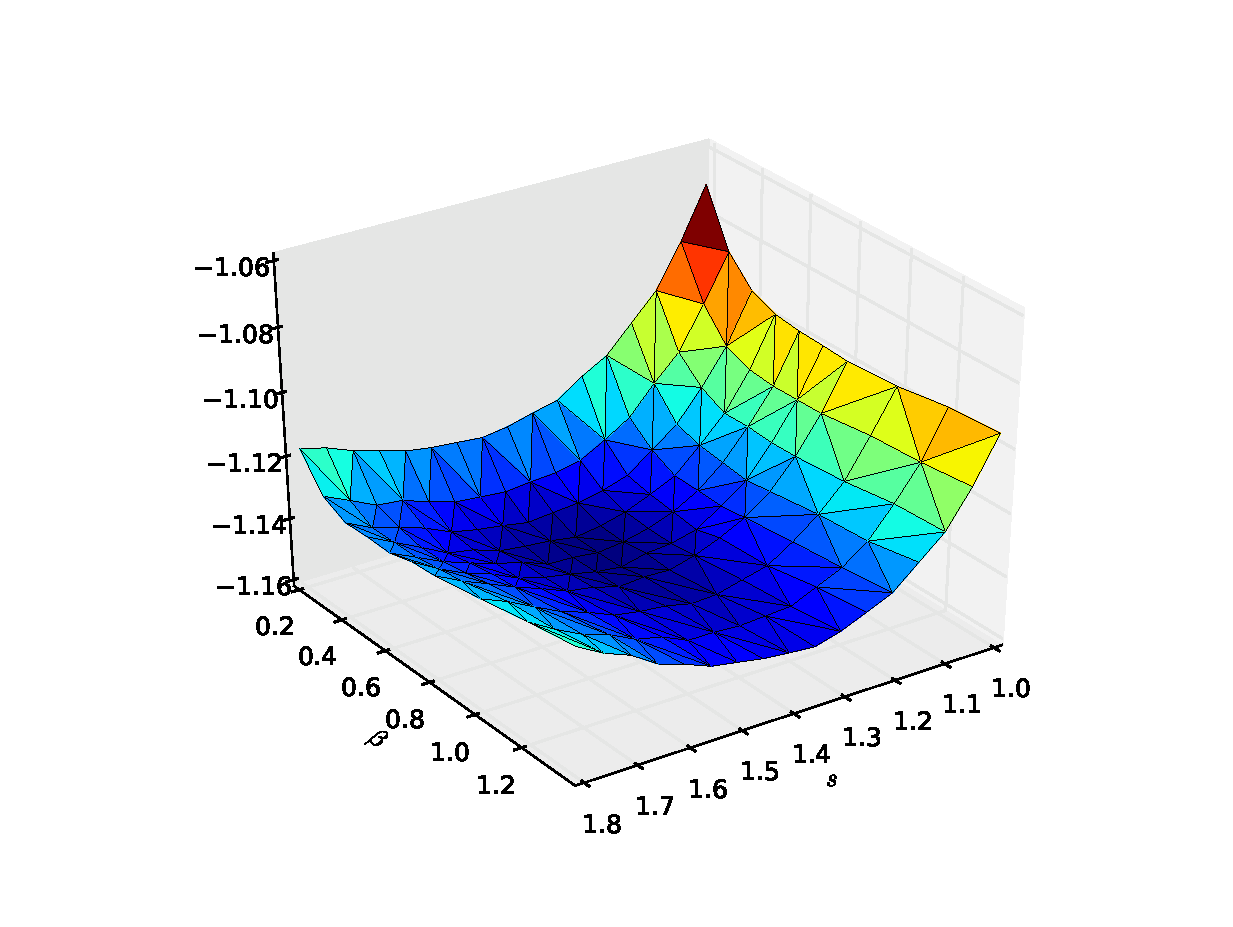
\includegraphics[width=\linewidth]{figs/3dPlot.eps}
\caption{3D plot of the energy $E$ as a function of both parameters $s$ and $beta$. We see the minimum at approximately $s\approx1.4$ and $\beta \approx 0.6$. This figure illustrates the dependence of the energy on the variational parameters. Observe a strong increase in energy for small $s$ and $\beta$. }
\label{fig:3dPlot}
\end{figure}

	
\section{Conclusions and look forward}
In this paper a variational Monte-Carlo method was used to obtain an estimation for the ground state wavefunction and energy of a hydrogen molecule. The result of $-1.1510 \pm 0.0003$ compared well to the experimental value $-1.1645$, but is highly dependent on the choice of variational wavefunction, which is a complex problem on its own. This paper therefore shows a proof of principle, that using Monte-Carlo integration in calculating the six dimensional integral in order to obtain the energy is a valid approach. The code is designed to be easily adopted to higher dimensional problems, for which the benefit of using Monte-Carlo integration increases due to the fact that the variance of the integral outcome goes as $\frac{1}{\sqrt{N}}$ and does not depend on the dimensions of the problem as opposed to equidistant integration methods.


\begin{thebibliography}{1}
	\bibitem{ref_Harju}
	A. Harju, S. Siljam\"aki, R. M. Nieminen (2002).
	\newblock Wigner molecules in quantum dots: A quantum Monte Carlo study,
	\newblock {\em Physical Review B. Volume 65, Issue 7. 075309/1-6.}
	
	\bibitem{ref_Thijssen}
	J. M. Thijssen (2007).
	\newblock Computational Physics, Ch. 10, 12,
	\newblock {\em Cambridge University Press}
	
	\bibitem{ref_NIST}
	B. Darwent (1970).
	\newblock Bond Dissociation Energies in Simple Molecules,
	\newblock{\em NIST NSRDS-NBS 31}
	
	\bibitem{ref_Grinter}
	R. Grinter (2005).
	\newblock The Quantum in Chemistry: An Experimentalist's View, Ch. 6
	\newblock {\em Wiley}
	
\end{thebibliography}
	
\end{document}
















